\documentclass[border=4pt]{standalone}
\usepackage{pgfplots}
\pgfplotsset{compat=1.17}
\usepackage{fontspec}
\setmainfont{Times New Roman}
\begin{document}
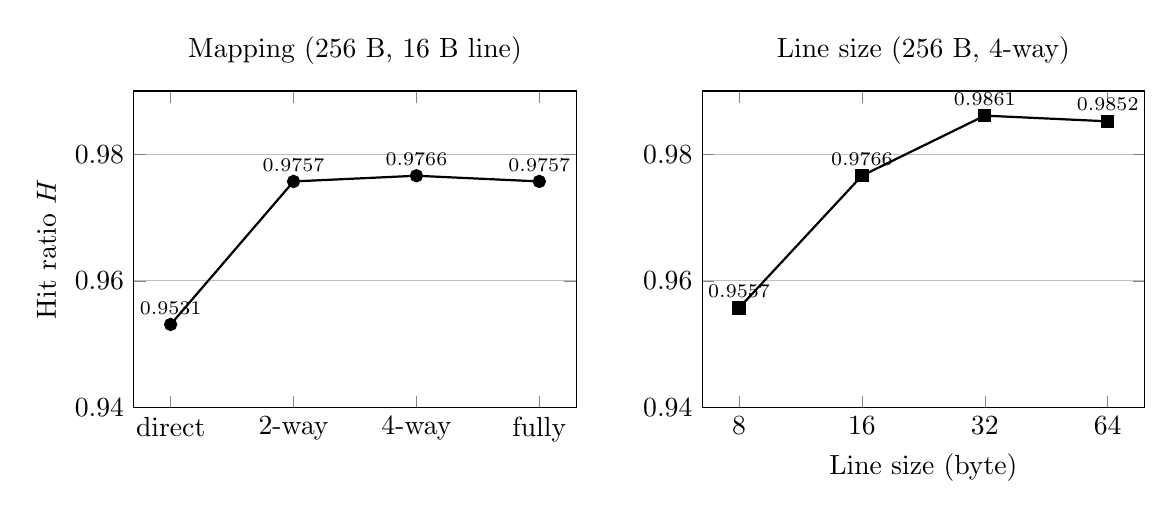
\begin{tikzpicture}
\begin{axis}[name=a, width=7.2cm, height=5.6cm, title={Mapping (256 B, 16 B line)},
  symbolic x coords={direct,2-way,4-way,fully}, xtick=data, ymin=0.94, ymax=0.99,
  ylabel={Hit ratio $H$}, ymajorgrids, nodes near coords, nodes near coords style={font=\scriptsize},
  every node near coord/.append style={/pgf/number format/.cd, fixed, precision=4}]
\addplot[mark=*, thick] coordinates {(direct,0.9531) (2-way,0.9757) (4-way,0.9766) (fully,0.9757)};
\end{axis}
\begin{axis}[at={(a.east)}, anchor=west, xshift=1.6cm, width=7.2cm, height=5.6cm,
  title={Line size (256 B, 4-way)}, xlabel={Line size (byte)},
  xtick={8,16,32,64}, xmode=log, log basis x=2, log ticks with fixed point, ymin=0.94, ymax=0.99,
  ymajorgrids, nodes near coords, nodes near coords style={font=\scriptsize},
  every node near coord/.append style={/pgf/number format/.cd, fixed, precision=4}]
\addplot[mark=square*, thick] coordinates {(8,0.9557) (16,0.9766) (32,0.9861) (64,0.9852)};
\end{axis}
\end{tikzpicture}
\end{document}
